\newpage
\section{Durchführung}
\label{sec:Durchfuehrung}
\begin{figure}
	\centering
	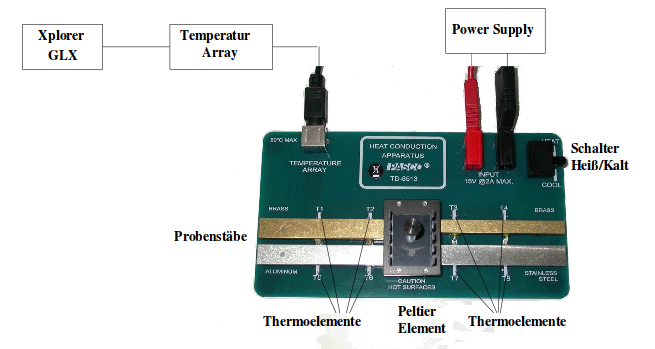
\includegraphics[width=\textwidth]{Bilder/Aufbau.png}
	\caption{Aufbau der Platine.}
\label{fig:platine}
\end{figure}
Um den zeitlichen Temperaturverlauf von vier Metallproben bestimmen zu können, wurden diese auf der in Abbildung \ref{fig:platine} gezeigten Platine angebracht. 
Mit dem mittig aufgesetzten Peltier-Element, bestehend aus zwei Halbleitern unterschiedlichen Energieniveaus, können die Stäbe durch Ausnutzen des Peltier-Effekts simultan geheizt oder gekühlt werden. 
Das Heizelement wird durch eine angeschlossene Spannungsquelle betrieben. 
An jedem Stab befinden sich zwei Thermoelemente, bestehend aus zwei metallischen Leitern, die an den Orten $x_1$ und $x_2$ die Temperaturen der Stäbe aufzeichnen. 
Dabei ruft die Temperaturdifferenz an den Thermoelementen gegensätzlich zum Peltier-Element, einen Spannungsunterschied hervor.
Durch Eichung kann die anliegende Spannung als Temperatur interpretiert und aufgenommen werden; hierzu wird ein Temperatur-Array und ein 
Datenlogger verwendet.

Vor Messbeginn werden sowohl die korrekte Verkabelung, als auch die Einstellungen des Datenloggers überprüft.
Alle acht Thermoelemente $T_\mathup{1}$ -- $T_\mathup{8}$ sollten eine Temperatur aufzeichnen.

\subsection{Statische Messung}

Das Peltier-Element wird mit einer Spannung $U_\mathup{P}=5 \si{\volt}$ bei maximalem Strom $I$ betrieben. 
Im Datenlogger wird eine Abtastrate von $\Delta{t}=5\si{\second}$ eingestellt. 
Nachdem die Isolierung auf die Probestäbe gelegt wurde, um einen Wärmeaustausch mit der Umgebung zu vermeiden, und der Schalter umgelegt ist, beginnt das Peltier-Element zu heizen. 
Der Datenlogger zeichnet alle 5 Sekunden die Temperaturen $T_i$, $i=1,..,8$ der Thermoelemente auf, bis Thermoelement $T_7$ eine Temperatur von $T_\mathup{7}\approx 43°C$ anzeigt. 
Anschließend werden die Isolierungen abgenommen, das Peltier-Element zum Kühlen der Stäbe auf den Modus "cool" gestellt.
%Die aufgenommenen Daten zur Auswertung auf einen USB-Stick übertragen und die für die Auswertung benötigten Diagramme des Temperaturverlaufs ausgedruckt.

\subsection{Dynamische Messung}
Nachdem die Stäbe auf eine Temperatur von $T<30°C$ gekühlt wurden, werden die Isolierungen erneut aufgelegt und das Peltier-Element beginnt bei einer Spannung von $U_\mathup{P}=8 \si{\volt}$ zu heizen. Die Thermoelemente zeichnen nun mit $\Delta{t}=2\si{\second}$ den Temperaturverlauf auf.

Nach $40\si\second$ wird das Peltier-Element umgeschaltet und die Stäbe für weitere $40\si\second$ gekühlt. 
Dieser Vorgang wird wiederholt, bis zehn Perioden von $T=80\si\second$ Dauer aufgezeichnet wurden. 
Anschließend werden die Stäbe analog zur statischen Messung wieder heruntergekühlt. 
Danach wird die dynamische Methode wiederholt, wobei die Periodendauer nun $T=200\si\second$ beträgt. 
%Erneut werden die Messdaten auf einen USB-Stick übertragen und einige Temperaturverläufe graphisch dargestellt und ausgedruckt.
